% Day 5: Risk, Regulation, and the Dark Side
% Complete Beamer slides for Digital Finance course
\documentclass[11pt,aspectratio=169]{beamer}
\usetheme{Madrid}

% ======================= PACKAGES =======================
\usepackage{graphicx}
\usepackage{booktabs}
\usepackage{adjustbox}
\usepackage{multicol}
\usepackage{amsmath}
\usepackage{amssymb}
\usepackage{tikz}
\usetikzlibrary{arrows,shapes,positioning,shadows,trees}
\usepackage{listings}
\usepackage{xcolor}

% ======================= COLOR DEFINITIONS =======================
% Primary color scheme: Blue/Teal for Digital Finance
\definecolor{dfblue}{RGB}{0,102,204}
\definecolor{dfteal}{RGB}{0,153,153}
\definecolor{dfcyan}{RGB}{51,187,204}
\definecolor{dflightblue}{RGB}{153,204,255}
\definecolor{dflightblue2}{RGB}{173,214,255}
\definecolor{dflightblue3}{RGB}{193,224,255}
\definecolor{dflightblue4}{RGB}{213,234,255}

% Accent colors for finance applications
\definecolor{dfgreen}{RGB}{44, 160, 44}
\definecolor{dfred}{RGB}{214, 39, 40}
\definecolor{dforange}{RGB}{255, 127, 14}
\definecolor{dfgray}{RGB}{127, 127, 127}

% Utility colors
\definecolor{lightgray}{RGB}{240, 240, 240}
\definecolor{midgray}{RGB}{180, 180, 180}
\definecolor{codebg}{RGB}{245, 245, 245}

% ======================= THEME CUSTOMIZATION =======================
% Apply Digital Finance color scheme to Madrid theme
\setbeamercolor{palette primary}{bg=dflightblue3,fg=dfblue}
\setbeamercolor{palette secondary}{bg=dflightblue2,fg=dfblue}
\setbeamercolor{palette tertiary}{bg=dfteal,fg=white}
\setbeamercolor{palette quaternary}{bg=dfblue,fg=white}

\setbeamercolor{structure}{fg=dfblue}
\setbeamercolor{section in toc}{fg=dfblue}
\setbeamercolor{subsection in toc}{fg=dfteal}
\setbeamercolor{title}{fg=dfblue}
\setbeamercolor{frametitle}{fg=dfblue,bg=dflightblue3}
\setbeamercolor{block title}{bg=dflightblue2,fg=dfblue}
\setbeamercolor{block body}{bg=dflightblue4,fg=black}

% Remove navigation symbols for cleaner look
\setbeamertemplate{navigation symbols}{}

% Clean itemize/enumerate
\setbeamertemplate{itemize items}[circle]
\setbeamertemplate{enumerate items}[default]

% Margins for readability
\setbeamersize{text margin left=8mm,text margin right=8mm}

% ======================= LISTINGS CONFIGURATION =======================
% Python code style
\lstdefinestyle{pythonstyle}{
    language=Python,
    basicstyle=\ttfamily\footnotesize,
    keywordstyle=\color{dfblue}\bfseries,
    stringstyle=\color{dforange},
    commentstyle=\color{dfgray}\itshape,
    numberstyle=\tiny\color{dfgray},
    numbers=left,
    numbersep=5pt,
    backgroundcolor=\color{codebg},
    showspaces=false,
    showstringspaces=false,
    showtabs=false,
    frame=single,
    rulecolor=\color{midgray},
    tabsize=4,
    captionpos=b,
    breaklines=true,
    breakatwhitespace=false,
    escapeinside={(*@}{@*)},
    xleftmargin=10pt,
    xrightmargin=10pt
}

% Solidity code style
\lstdefinestyle{soliditystyle}{
    language=Java, % closest approximation
    basicstyle=\ttfamily\footnotesize,
    keywordstyle=\color{dfteal}\bfseries,
    stringstyle=\color{dforange},
    commentstyle=\color{dfgray}\itshape,
    numberstyle=\tiny\color{dfgray},
    numbers=left,
    numbersep=5pt,
    backgroundcolor=\color{codebg},
    showspaces=false,
    showstringspaces=false,
    showtabs=false,
    frame=single,
    rulecolor=\color{midgray},
    tabsize=2,
    captionpos=b,
    breaklines=true,
    breakatwhitespace=false,
    escapeinside={(*@}{@*)},
    xleftmargin=10pt,
    xrightmargin=10pt,
    morekeywords={pragma, contract, function, returns, public, private, view, pure, payable, address, uint256, mapping, event, modifier}
}

% Inline code command
\newcommand{\code}[1]{\texttt{\color{dfblue}#1}}

% ======================= CUSTOM COMMANDS =======================
% Bottom annotation (Madrid-style)
\newcommand{\bottomnote}[1]{%
\vfill
\vspace{-2mm}
\textcolor{dflightblue2}{\rule{\textwidth}{0.4pt}}
\vspace{1mm}
\footnotesize
\textbf{#1}
}

% Compact list spacing
\newcommand{\compactlist}{%
\setlength{\itemsep}{0pt}%
\setlength{\parskip}{0pt}%
\setlength{\parsep}{0pt}%
}

% Chart placeholder
\newcommand{\chartplaceholder}[2][5cm]{%
\begin{center}
\begin{adjustbox}{max width=0.95\textwidth, max height=#1}
\framebox[\textwidth][c]{%
\rule{0pt}{#1}%
\textcolor{midgray}{[#2]}%
}
\end{adjustbox}
\end{center}
}

% ======================= FINANCE NOTATION MACROS =======================
% Probability and statistics
\newcommand{\E}{\mathbb{E}} % Expected value
\newcommand{\Var}{\mathrm{Var}} % Variance
\newcommand{\Cov}{\mathrm{Cov}} % Covariance
\newcommand{\Prob}{\mathbb{P}} % Probability

% Distributions
\newcommand{\Normal}{\mathcal{N}} % Normal distribution
\newcommand{\Uniform}{\mathcal{U}} % Uniform distribution

% Returns and prices
\newcommand{\Ret}{R} % Return
\newcommand{\LogRet}{r} % Log return
\newcommand{\Price}{S} % Price/Stock price
\newcommand{\Strike}{K} % Strike price

% Options and derivatives
\newcommand{\CallPrice}{C} % Call option price
\newcommand{\PutPrice}{P} % Put option price
\newcommand{\Greeks}[1]{\mathit{#1}} % Greek letters

% Risk measures
\newcommand{\VaR}{\mathrm{VaR}} % Value at Risk
\newcommand{\CVaR}{\mathrm{CVaR}} % Conditional VaR
\newcommand{\Sharpe}{\mathrm{SR}} % Sharpe Ratio

% Time series
\newcommand{\AR}{\mathrm{AR}} % Autoregressive
\newcommand{\MA}{\mathrm{MA}} % Moving average
\newcommand{\GARCH}{\mathrm{GARCH}} % GARCH

% Blockchain/Crypto
\newcommand{\Hash}{\mathrm{Hash}} % Hash function
\newcommand{\Block}{\mathcal{B}} % Block
\newcommand{\Chain}{\mathcal{C}} % Chain

% Real numbers, integers
\newcommand{\R}{\mathbb{R}}
\newcommand{\Z}{\mathbb{Z}}
\newcommand{\N}{\mathbb{N}}

% ======================= TIKZ STYLES =======================
% Styles for finance-related diagrams
\tikzstyle{process} = [rectangle, minimum width=3cm, minimum height=1cm, text centered, draw=dfblue, fill=dflightblue4, thick]
\tikzstyle{decision} = [diamond, minimum width=3cm, minimum height=1cm, text centered, draw=dfteal, fill=dflightblue4, thick]
\tikzstyle{arrow} = [thick,->,>=stealth,color=dfblue]
\tikzstyle{blockchain} = [rectangle, rounded corners, minimum width=2.5cm, minimum height=1cm, text centered, draw=dfteal, fill=dflightblue3, thick]
\tikzstyle{transaction} = [circle, minimum size=0.8cm, text centered, draw=dforange, fill=dflightblue4, thick]

% ======================= FOOTER TEMPLATE =======================
\setbeamertemplate{footline}{
    \hbox{\begin{beamercolorbox}[wd=\paperwidth,ht=2.5ex,dp=1ex,leftskip=.5em,rightskip=.5em]{author in head/foot}
    \tiny
    \textbf{Digital Finance} \hfill
    Joerg Osterrieder \hfill
    \insertdate \hfill
    Page \insertframenumber{} / \inserttotalframenumber
    \end{beamercolorbox}}
}

% ======================= SECTION DIVIDER TEMPLATE =======================
\AtBeginSection[]{
\begin{frame}[plain]
\vfill
\centering
\begin{beamercolorbox}[sep=12pt,center]{title}
\usebeamerfont{title}\LARGE\insertsection\par
\end{beamercolorbox}
\vfill
\end{frame}
}


% ======================= DOCUMENT INFO =======================
\title[Day 5: Risk, Regulation, and the Dark Side]{Day 5: Risk, Regulation, and the Dark Side}
\subtitle{What Goes Wrong and Who Decides What's Allowed}
\author{Joerg Osterrieder}
\institute{Digital Finance}
\date{2025}

\begin{document}

% ======================= TITLE SLIDE =======================
\begin{frame}[plain]
\titlepage
\end{frame}

% ======================= DAY OVERVIEW =======================
\begin{frame}{Today's Journey}
\begin{columns}[T]
\begin{column}{0.48\textwidth}
\textbf{Where We're Going:}
\begin{itemize}
\item What fails in digital finance?
\item How do governments respond?
\item Who governs decentralized systems?
\item Who benefits and who is harmed?
\end{itemize}
\end{column}
\begin{column}{0.48\textwidth}
\textbf{By Day's End, You Will:}
\begin{itemize}
\item Categorize failure modes and exploits
\item Compare regulatory frameworks globally
\item Evaluate DAO governance tradeoffs
\item Form positions on privacy vs. surveillance
\end{itemize}
\end{column}
\end{columns}

\vspace{5mm}
\begin{center}
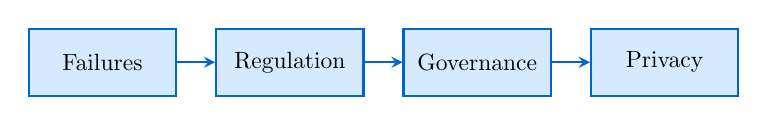
\begin{tikzpicture}[node distance=2.8cm, scale=0.85, transform shape]
\node (failures) [process, minimum width=2.2cm] {Failures};
\node (regulation) [process, right of=failures, minimum width=2.2cm] {Regulation};
\node (governance) [process, right of=regulation, minimum width=2.2cm] {Governance};
\node (privacy) [process, right of=governance, minimum width=2.2cm] {Privacy};
\draw [arrow] (failures) -- (regulation);
\draw [arrow] (regulation) -- (governance);
\draw [arrow] (governance) -- (privacy);
\end{tikzpicture}
\end{center}
\end{frame}

% =====================================================================
% SECTION 5.1: WHAT GOES WRONG
% =====================================================================
\section{5.1 What Goes Wrong}

\begin{frame}{Topic 5.1: What Goes Wrong}
\begin{center}
\textbf{\Large Failures, Hacks, and Systemic Risk in Digital Finance}
\end{center}

\vspace{5mm}
\textbf{Learning Objectives:}
\begin{itemize}
\item Categorize types of digital finance failures
\item Explain mechanics of major exploit types
\item Assess systemic risk implications
\item Develop genuine risk awareness
\end{itemize}

\vspace{5mm}
\begin{block}{Hands-On Component}
Colab notebook (NB11) simulating historical DeFi exploits---run reentrancy, flash loan, and oracle manipulation scenarios to understand how attacks work.
\end{block}
\end{frame}

\begin{frame}{A Taxonomy of Failures}
\begin{center}
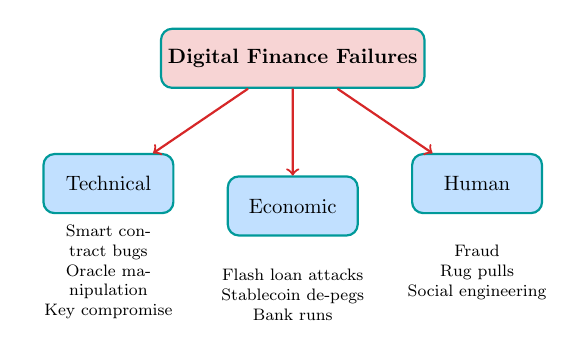
\begin{tikzpicture}[scale=0.75, transform shape]
% Main categories
\node (failures) [blockchain, minimum width=3cm, fill=dfred!20] {\textbf{Digital Finance Failures}};

\node (technical) [blockchain, below left of=failures, node distance=3cm, xshift=-1cm, minimum width=2.2cm] {Technical};
\node (economic) [blockchain, below of=failures, node distance=2.5cm, minimum width=2.2cm] {Economic};
\node (human) [blockchain, below right of=failures, node distance=3cm, xshift=1cm, minimum width=2.2cm] {Human};

% Arrows
\draw[->, thick, dfred] (failures) -- (technical);
\draw[->, thick, dfred] (failures) -- (economic);
\draw[->, thick, dfred] (failures) -- (human);

% Sub-categories
\node[below of=technical, node distance=1.5cm, font=\footnotesize, text width=2.5cm, align=center] {Smart contract bugs\\Oracle manipulation\\Key compromise};

\node[below of=economic, node distance=1.5cm, font=\footnotesize, text width=2.5cm, align=center] {Flash loan attacks\\Stablecoin de-pegs\\Bank runs};

\node[below of=human, node distance=1.5cm, font=\footnotesize, text width=2.5cm, align=center] {Fraud\\Rug pulls\\Social engineering};
\end{tikzpicture}
\end{center}
\end{frame}

\begin{frame}{Category 1: Technical Failures}
\begin{columns}[T]
\begin{column}{0.48\textwidth}
\textbf{Smart Contract Bugs:}
\begin{itemize}
\item Reentrancy attacks
\item Integer overflow/underflow
\item Logic errors
\item Access control flaws
\end{itemize}

\vspace{3mm}
\textbf{Infrastructure Failures:}
\begin{itemize}
\item Oracle manipulation
\item Bridge vulnerabilities
\item Consensus bugs
\item Key management failures
\end{itemize}
\end{column}
\begin{column}{0.48\textwidth}
\begin{alertblock}{The DAO Hack (2016)}
\textbf{Loss:} \$60M (3.6M ETH)\\
\textbf{Cause:} Reentrancy bug\\
\textbf{Result:} Ethereum hard fork\\
\textbf{Lesson:} Code is NOT always law
\end{alertblock}

\vspace{3mm}
\begin{block}{Wormhole Bridge (2022)}
\textbf{Loss:} \$320M\\
\textbf{Cause:} Signature verification bug\\
Attacker minted unbacked tokens
\end{block}
\end{column}
\end{columns}
\end{frame}

\begin{frame}{Deep Dive: Reentrancy Attack}
\begin{center}
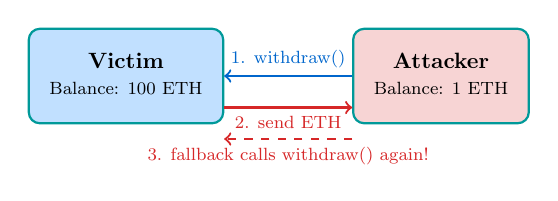
\begin{tikzpicture}[scale=0.8, transform shape, node distance=2cm]
% Victim contract
\node (victim) [blockchain, minimum width=2.5cm, minimum height=1.5cm] {
\begin{tabular}{c}
\textbf{Victim}\\
\footnotesize Balance: 100 ETH
\end{tabular}
};

% Attacker contract
\node (attacker) [blockchain, right of=victim, node distance=5cm, minimum width=2.5cm, minimum height=1.5cm, fill=dfred!20] {
\begin{tabular}{c}
\textbf{Attacker}\\
\footnotesize Balance: 1 ETH
\end{tabular}
};

% Steps
\draw[->, thick, dfblue] (attacker.west) -- node[above, font=\footnotesize] {1. withdraw()} (victim.east);
\draw[->, thick, dfred] ([yshift=-5mm]victim.east) -- node[below, font=\footnotesize] {2. send ETH} ([yshift=-5mm]attacker.west);
\draw[->, thick, dfred, dashed] ([yshift=-10mm]attacker.west) -- node[below, font=\footnotesize] {3. fallback calls withdraw() again!} ([yshift=-10mm]victim.east);

\end{tikzpicture}
\end{center}

\vspace{3mm}
\textbf{The Problem:}
\begin{enumerate}
\item Victim sends ETH \textit{before} updating balance
\item Attacker's fallback function calls withdraw() again
\item Balance not yet updated, so check passes again
\item Repeat until contract drained
\end{enumerate}

\begin{block}{Prevention}
Check-Effects-Interactions pattern: Update state BEFORE external calls.
\end{block}
\end{frame}

\begin{frame}{Reentrancy: Vulnerable vs. Safe (Pseudocode)}
\begin{columns}[T]
\begin{column}{0.48\textwidth}
\textbf{Vulnerable Process:}
\begin{enumerate}
\item Check: Does user have a balance? \textcolor{dfgreen}{\checkmark}
\item \textcolor{dfred}{\textbf{Send money to user}}
\item[] \textcolor{dfred}{$\to$ Attacker calls back HERE}
\item[] \textcolor{dfred}{$\to$ Repeat step 2 (loop!)}
\item Update records: set balance to 0
\item[] \textcolor{dfred}{$\to$ Too late---money already sent multiple times!}
\end{enumerate}
\end{column}
\begin{column}{0.48\textwidth}
\textbf{Safe Process:}
\begin{enumerate}
\item Check: Does user have a balance? \textcolor{dfgreen}{\checkmark}
\item \textcolor{dfgreen}{\textbf{Update records FIRST:}} set balance to 0
\item \textcolor{dfgreen}{\textbf{Then send money}}
\item[] \textcolor{dfgreen}{$\to$ If attacker calls back, balance is already 0}
\item[] \textcolor{dfgreen}{$\to$ Attack fails!}
\end{enumerate}
\end{column}
\end{columns}

\vspace{3mm}
\begin{alertblock}{Check-Effects-Interactions Pattern}
\begin{enumerate}
\item \textbf{Check:} Validate conditions (is the request valid?)
\item \textbf{Effects:} Update your records (mark as done)
\item \textbf{Interactions:} Send money last (external calls at the end)
\end{enumerate}
\end{alertblock}
\end{frame}

\begin{frame}{Category 2: Economic Attacks}
\begin{columns}[T]
\begin{column}{0.48\textwidth}
\textbf{Flash Loan Attacks:}
\begin{itemize}
\item Borrow millions, attack, repay---all in one transaction
\item No collateral needed
\item Exploit price discrepancies
\item Manipulate governance votes
\end{itemize}

\vspace{3mm}
\textbf{How Flash Loans Work:}
\begin{enumerate}
\item Borrow \$100M (uncollateralized)
\item Execute attack strategy
\item Repay \$100M + fee
\item If any step fails, entire tx reverts
\end{enumerate}
\end{column}
\begin{column}{0.48\textwidth}
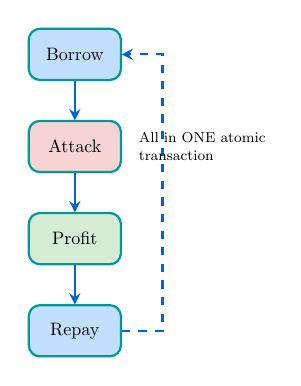
\begin{tikzpicture}[scale=0.65, transform shape, node distance=1.8cm]
% Flash loan cycle
\node (borrow) [blockchain, minimum width=1.8cm] {Borrow};
\node (attack) [blockchain, below of=borrow, minimum width=1.8cm, fill=dfred!20] {Attack};
\node (profit) [blockchain, below of=attack, minimum width=1.8cm, fill=dfgreen!20] {Profit};
\node (repay) [blockchain, below of=profit, minimum width=1.8cm] {Repay};

\draw[arrow] (borrow) -- (attack);
\draw[arrow] (attack) -- (profit);
\draw[arrow] (profit) -- (repay);
\draw[arrow, dashed] (repay.east) -- ++(0.8,0) |- (borrow.east);

\node[right of=attack, node distance=2.5cm, font=\footnotesize, text width=2.5cm] {All in ONE atomic transaction};
\end{tikzpicture}
\end{column}
\end{columns}
\end{frame}

\begin{frame}{Flash Loan Attack Example: bZx (2020)}
\begin{center}
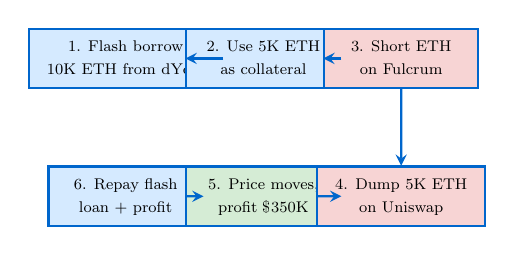
\begin{tikzpicture}[scale=0.7, transform shape, node distance=2.5cm]
% Steps
\node (step1) [process, minimum width=2.8cm, minimum height=1cm] {
\begin{tabular}{c}
\footnotesize 1. Flash borrow\\
\footnotesize 10K ETH from dYdX
\end{tabular}
};

\node (step2) [process, right of=step1, minimum width=2.8cm, minimum height=1cm] {
\begin{tabular}{c}
\footnotesize 2. Use 5K ETH\\
\footnotesize as collateral
\end{tabular}
};

\node (step3) [process, right of=step2, minimum width=2.8cm, minimum height=1cm, fill=dfred!20] {
\begin{tabular}{c}
\footnotesize 3. Short ETH\\
\footnotesize on Fulcrum
\end{tabular}
};

\node (step4) [process, below of=step1, minimum width=2.8cm, minimum height=1cm] {
\begin{tabular}{c}
\footnotesize 6. Repay flash\\
\footnotesize loan + profit
\end{tabular}
};

\node (step5) [process, below of=step2, minimum width=2.8cm, minimum height=1cm, fill=dfgreen!20] {
\begin{tabular}{c}
\footnotesize 5. Price moves,\\
\footnotesize profit \$350K
\end{tabular}
};

\node (step6) [process, below of=step3, minimum width=2.8cm, minimum height=1cm, fill=dfred!20] {
\begin{tabular}{c}
\footnotesize 4. Dump 5K ETH\\
\footnotesize on Uniswap
\end{tabular}
};

% Arrows
\draw[arrow] (step1) -- (step2);
\draw[arrow] (step2) -- (step3);
\draw[arrow] (step3) -- (step6);
\draw[arrow] (step6) -- (step5);
\draw[arrow] (step5) -- (step4);
\end{tikzpicture}
\end{center}

\vspace{3mm}
\textbf{Key insight:} Capital requirement to manipulate markets dropped from millions to \textbf{zero}.
\end{frame}

\begin{frame}{Category 3: Stablecoin Failures}
\begin{columns}[T]
\begin{column}{0.55\textwidth}
\textbf{UST/LUNA Collapse (May 2022):}
\begin{itemize}
\item Algorithmic stablecoin
\item Market cap: \$18B at peak
\item De-pegged from \$1 to \$0.10
\item LUNA: \$80 to \$0.0001
\item Total value destroyed: \$40B+
\end{itemize}

\vspace{3mm}
\textbf{The Death Spiral:}
\begin{enumerate}
\item Large UST sell-off
\item Peg breaks, panic ensues
\item LUNA minted to defend peg
\item LUNA hyperinflates
\item Both collapse to zero
\end{enumerate}
\end{column}
\begin{column}{0.42\textwidth}
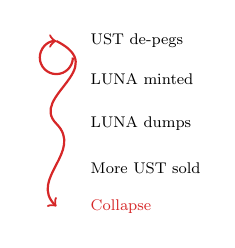
\begin{tikzpicture}[scale=0.7, transform shape]
% Death spiral
\draw[thick, dfred, ->] (0,3) .. controls (1,2.5) and (-0.5,2) .. (0,1.5) .. controls (0.5,1) and (-0.5,0.5) .. (0,0);

\node[right] at (0.5,3) {\footnotesize UST de-pegs};
\node[right] at (0.5,2.3) {\footnotesize LUNA minted};
\node[right] at (0.5,1.5) {\footnotesize LUNA dumps};
\node[right] at (0.5,0.7) {\footnotesize More UST sold};
\node[right] at (0.5,0) {\footnotesize \textcolor{dfred}{Collapse}};

% Spiral arrow indicating loop
\draw[thick, dfred, ->] (0.3,2.7) arc (0:-270:0.3);
\end{tikzpicture}

\vspace{3mm}
\begin{alertblock}{Lesson}
Algorithmic stability requires robust mechanisms---``code'' alone is insufficient.
\end{alertblock}
\end{column}
\end{columns}
\end{frame}

\begin{frame}{Category 4: Centralized Exchange Collapses}
\begin{columns}[T]
\begin{column}{0.48\textwidth}
\textbf{FTX Collapse (Nov 2022):}
\begin{itemize}
\item 2nd largest crypto exchange
\item \$32B valuation
\item Customer funds misappropriated
\item \$8B+ missing
\item CEO convicted of fraud
\end{itemize}

\vspace{3mm}
\textbf{Mt. Gox (2014):}
\begin{itemize}
\item 70\% of Bitcoin trading
\item 850,000 BTC ``lost''
\item Combination of hack + fraud
\item 10+ years to partial recovery
\end{itemize}
\end{column}
\begin{column}{0.48\textwidth}
\textbf{Common Patterns:}
\begin{enumerate}
\item Opaque operations
\item Commingled funds
\item Lack of proof of reserves
\item Regulatory arbitrage
\item Charismatic founders
\end{enumerate}

\vspace{3mm}
\begin{alertblock}{Not Your Keys, Not Your Coins}
Centralized custodians reintroduce the trust problems DeFi was designed to solve.
\end{alertblock}
\end{column}
\end{columns}
\end{frame}

\begin{frame}{Category 5: Rug Pulls and Fraud}
\begin{columns}[T]
\begin{column}{0.55\textwidth}
\textbf{Types of Rug Pulls:}
\begin{itemize}
\item \textbf{Liquidity pull:} Developers drain LP tokens
\item \textbf{Limiting sell orders:} Hidden code prevents selling
\item \textbf{Dumping:} Team sells massive holdings
\item \textbf{Exit scam:} Project disappears with funds
\end{itemize}

\vspace{3mm}
\textbf{Red Flags:}
\begin{itemize}
\item Anonymous team
\item Unlocked liquidity
\item No audit
\item Unrealistic promises
\item FOMO marketing
\item Celebrity endorsements
\end{itemize}
\end{column}
\begin{column}{0.42\textwidth}
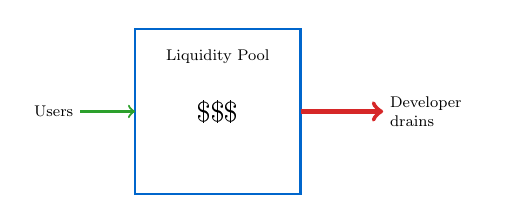
\begin{tikzpicture}[scale=0.7, transform shape]
% Rug pull diagram
\draw[thick, dfblue] (0,0) -- (0,3) -- (3,3) -- (3,0) -- cycle;
\node at (1.5,2.5) {\footnotesize Liquidity Pool};

% Users depositing
\draw[->, thick, dfgreen] (-1,1.5) -- (0,1.5);
\node[left, font=\footnotesize] at (-1,1.5) {Users};

% Rug pull
\draw[->, ultra thick, dfred] (3,1.5) -- (4.5,1.5);
\node[right, font=\footnotesize, text width=1.5cm] at (4.5,1.5) {Developer drains};

% Money icons
\node at (1.5,1.5) {\Large \$\$\$};
\end{tikzpicture}

\vspace{5mm}
\textbf{2021 Stats:}\\
\$2.8B lost to rug pulls\\
(Chainalysis)
\end{column}
\end{columns}
\end{frame}

\begin{frame}{Systemic Risk in Digital Finance}
\begin{center}
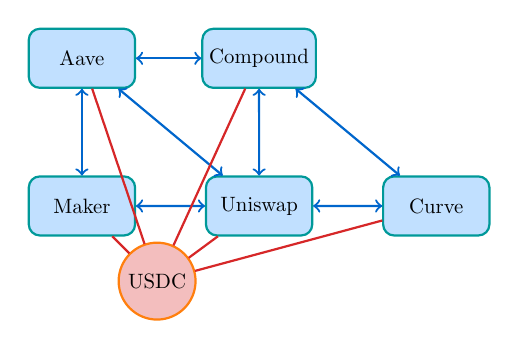
\begin{tikzpicture}[scale=0.75, transform shape]
% Interconnected protocols
\node (aave) [blockchain, minimum width=1.8cm] {Aave};
\node (compound) [blockchain, right of=aave, node distance=3cm, minimum width=1.8cm] {Compound};
\node (maker) [blockchain, below of=aave, node distance=2.5cm, minimum width=1.8cm] {Maker};
\node (uniswap) [blockchain, below of=compound, node distance=2.5cm, minimum width=1.8cm] {Uniswap};
\node (curve) [blockchain, right of=uniswap, node distance=3cm, minimum width=1.8cm] {Curve};

% Connections
\draw[thick, dfblue, <->] (aave) -- (compound);
\draw[thick, dfblue, <->] (aave) -- (maker);
\draw[thick, dfblue, <->] (compound) -- (uniswap);
\draw[thick, dfblue, <->] (maker) -- (uniswap);
\draw[thick, dfblue, <->] (uniswap) -- (curve);
\draw[thick, dfblue, <->] (aave) -- (uniswap);
\draw[thick, dfblue, <->] (compound) -- (curve);

% Stablecoins at center
\node (usdc) [transaction, below right of=maker, node distance=1.8cm, fill=dfred!30] {USDC};
\draw[thick, dfred] (usdc) -- (aave);
\draw[thick, dfred] (usdc) -- (compound);
\draw[thick, dfred] (usdc) -- (maker);
\draw[thick, dfred] (usdc) -- (uniswap);
\draw[thick, dfred] (usdc) -- (curve);
\end{tikzpicture}
\end{center}

\vspace{3mm}
\textbf{DeFi Composability = Systemic Risk:}
\begin{itemize}
\item Protocols depend on each other (``money legos'')
\item Stablecoins are systemic (USDC freeze = cascade)
\item Oracle failure affects ALL dependent protocols
\item Smart contract bug can propagate through ecosystem
\end{itemize}
\end{frame}

\begin{frame}{Largest DeFi Exploits (2020-2024)}
\begin{center}
\renewcommand{\arraystretch}{1.3}
\begin{tabular}{|l|r|l|l|}
\hline
\textbf{Protocol} & \textbf{Loss} & \textbf{Type} & \textbf{Year} \\
\hline
Ronin Bridge & \$625M & Bridge exploit & 2022 \\
\hline
Poly Network & \$611M & Bridge exploit & 2021 \\
\hline
FTX & \$477M & Hack post-bankruptcy & 2022 \\
\hline
Wormhole & \$320M & Bridge exploit & 2022 \\
\hline
Nomad Bridge & \$190M & Bridge exploit & 2022 \\
\hline
Beanstalk & \$182M & Flash loan governance & 2022 \\
\hline
Wintermute & \$160M & Key compromise & 2022 \\
\hline
\end{tabular}
\end{center}

\vspace{3mm}
\begin{alertblock}{Pattern Recognition}
\textbf{Bridges are the weakest link.} Cross-chain bridges hold massive TVL but have complex attack surfaces.
\end{alertblock}
\end{frame}

\begin{frame}{Hands-On: Analyzing an Exploit (NB11)}
\begin{center}
\textbf{\Large Simulate Real Exploit Scenarios}
\end{center}

\vspace{5mm}
\textbf{In the Colab notebook, we will:}
\begin{enumerate}
\item Run simulations of exploit scenarios (reentrancy, flash loans, oracle manipulation)
\item Model how each attack type drains funds step-by-step
\item Identify the attack patterns and vulnerabilities
\item Calculate attacker profit in simulated scenarios
\item Discuss what could have prevented each exploit
\end{enumerate}

\vspace{5mm}
\begin{block}{Access the Notebook}
\texttt{day\_05/notebooks/NB11\_DeFi\_Exploits.ipynb}

\vspace{2mm}
\footnotesize We'll simulate real exploit types to understand how they work.
\end{block}

\bottomnote{Time: 20-25 minutes for guided exploration}
\end{frame}

\begin{frame}{Discussion: Risk Awareness}
\begin{columns}[T]
\begin{column}{0.48\textwidth}
\textbf{Questions to Consider:}
\begin{enumerate}
\item Should smart contracts be audited before deployment?
\item Who is liable when code fails?
\item Is ``code is law'' a feature or a bug?
\item How do we balance innovation with safety?
\end{enumerate}
\end{column}
\begin{column}{0.48\textwidth}
\textbf{Key Takeaways:}
\begin{itemize}
\item Failures are inevitable---design for them
\item Technical, economic, and human risks compound
\item Transparency enables post-mortem but not prevention
\item Systemic risk grows with interconnection
\end{itemize}
\end{column}
\end{columns}

\vspace{5mm}
\begin{alertblock}{Risk Framework}
For any protocol: What can go wrong technically? Economically? Who has the keys? What happens when it fails?
\end{alertblock}
\end{frame}

% =====================================================================
% SECTION 5.2: REGULATORY LANDSCAPES
% =====================================================================
\section{5.2 Regulatory Landscapes}

\begin{frame}{Topic 5.2: Regulatory Landscapes}
\begin{center}
\textbf{\Large How Governments Respond to Digital Finance}
\end{center}

\vspace{5mm}
\textbf{Learning Objectives:}
\begin{itemize}
\item Compare major regulatory frameworks (US, EU, Asia)
\item Explain policy rationale behind key regulations
\item Predict how regulation shapes innovation trajectories
\item Understand why the same technology gets treated differently
\end{itemize}

\vspace{5mm}
\begin{block}{Why Regulation Matters}
Regulation determines which innovations survive. Understanding regulatory logic helps you build compliant products and predict market evolution.
\end{block}
\end{frame}

\begin{frame}{The Regulatory Challenge}
\begin{columns}[T]
\begin{column}{0.48\textwidth}
\textbf{What regulators want:}
\begin{itemize}
\item Consumer protection
\item Market integrity
\item Financial stability
\item Anti-money laundering
\item Tax compliance
\item National security
\end{itemize}
\end{column}
\begin{column}{0.48\textwidth}
\textbf{What innovators want:}
\begin{itemize}
\item Permissionless access
\item Privacy
\item Speed to market
\item Global reach
\item Minimal compliance costs
\item Regulatory clarity
\end{itemize}
\end{column}
\end{columns}

\vspace{5mm}
\begin{center}
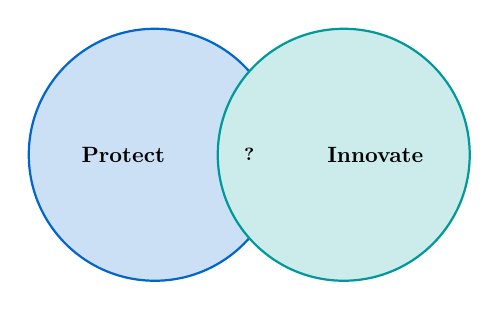
\begin{tikzpicture}[scale=0.8, transform shape]
\draw[thick, dfblue, fill=dfblue!20] (0,0) circle (2cm);
\draw[thick, dfteal, fill=dfteal!20] (3,0) circle (2cm);

\node at (-0.5,0) {\textbf{Protect}};
\node at (3.5,0) {\textbf{Innovate}};
\node at (1.5,0) {\footnotesize \textbf{?}};
\end{tikzpicture}
\end{center}
\end{frame}

\begin{frame}{United States: Fragmented Landscape}
\begin{center}
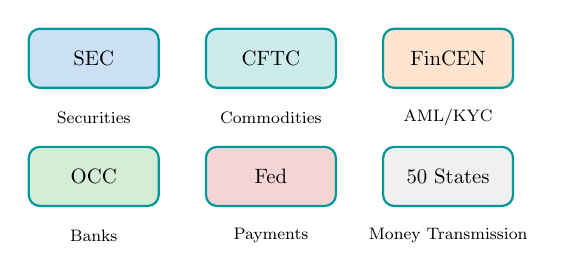
\begin{tikzpicture}[scale=0.75, transform shape]
% Regulatory agencies
\node (sec) [blockchain, minimum width=2.2cm, fill=dfblue!20] {SEC};
\node (cftc) [blockchain, right of=sec, node distance=3cm, minimum width=2.2cm, fill=dfteal!20] {CFTC};
\node (fincen) [blockchain, right of=cftc, node distance=3cm, minimum width=2.2cm, fill=dforange!20] {FinCEN};
\node (occ) [blockchain, below of=sec, node distance=2cm, minimum width=2.2cm, fill=dfgreen!20] {OCC};
\node (fed) [blockchain, below of=cftc, node distance=2cm, minimum width=2.2cm, fill=dfred!20] {Fed};
\node (state) [blockchain, below of=fincen, node distance=2cm, minimum width=2.2cm, fill=lightgray] {50 States};

% Labels
\node[below of=sec, node distance=1cm, font=\footnotesize] {Securities};
\node[below of=cftc, node distance=1cm, font=\footnotesize] {Commodities};
\node[below of=fincen, node distance=1cm, font=\footnotesize] {AML/KYC};
\node[below of=occ, node distance=1cm, font=\footnotesize] {Banks};
\node[below of=fed, node distance=1cm, font=\footnotesize] {Payments};
\node[below of=state, node distance=1cm, font=\footnotesize] {Money Transmission};
\end{tikzpicture}
\end{center}

\vspace{3mm}
\textbf{Key issue:} No single regulator. Turf wars between SEC and CFTC.
\end{frame}

\begin{frame}{US: The Howey Test}
\begin{columns}[T]
\begin{column}{0.55\textwidth}
\textbf{Is it a security?}\\
A token is a security if it involves:
\begin{enumerate}
\item \textbf{Investment of money}
\item \textbf{In a common enterprise}
\item \textbf{With expectation of profits}
\item \textbf{Derived from others' efforts}
\end{enumerate}

\vspace{3mm}
\textbf{SEC Position:}
\begin{itemize}
\item Most ICOs were securities
\item Many tokens are securities
\item ETH and BTC are NOT securities
\item ``Come in and register''
\end{itemize}
\end{column}
\begin{column}{0.42\textwidth}
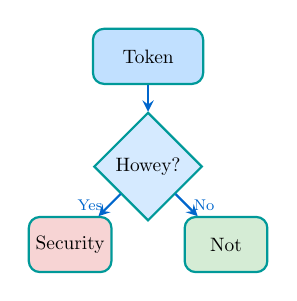
\begin{tikzpicture}[scale=0.7, transform shape]
% Decision tree
\node (start) [blockchain, minimum width=2cm] {Token};
\node (howey) [decision, below of=start, node distance=2cm, minimum width=1.5cm, minimum height=1.5cm] {Howey?};
\node (security) [blockchain, below left of=howey, node distance=2cm, fill=dfred!20, minimum width=1.5cm] {Security};
\node (commodity) [blockchain, below right of=howey, node distance=2cm, fill=dfgreen!20, minimum width=1.5cm] {Not};

\draw[arrow] (start) -- (howey);
\draw[arrow] (howey) -- node[left, font=\footnotesize] {Yes} (security);
\draw[arrow] (howey) -- node[right, font=\footnotesize] {No} (commodity);
\end{tikzpicture}

\vspace{3mm}
\textbf{Consequences:}\\
\footnotesize Securities require registration, prospectus, qualified investors only.
\end{column}
\end{columns}
\end{frame}

\begin{frame}{US Enforcement Actions (2023-2024)}
\begin{center}
\renewcommand{\arraystretch}{1.3}
\begin{tabular}{|l|l|p{5cm}|}
\hline
\textbf{Target} & \textbf{Allegation} & \textbf{Status} \\
\hline
Coinbase & Operating unregistered exchange & Ongoing litigation \\
\hline
Binance & Multiple securities violations & \$4.3B settlement \\
\hline
Kraken & Unregistered staking service & \$30M settlement \\
\hline
Ripple (XRP) & Unregistered securities & Partial win for Ripple \\
\hline
Terraform & Securities fraud (UST) & Founders charged \\
\hline
\end{tabular}
\end{center}

\vspace{3mm}
\begin{alertblock}{Regulation by Enforcement}
US lacks comprehensive crypto legislation. SEC and CFTC establish rules through lawsuits rather than clear guidelines.
\end{alertblock}
\end{frame}

\begin{frame}{European Union: MiCA Framework}
\begin{columns}[T]
\begin{column}{0.55\textwidth}
\textbf{Markets in Crypto-Assets (MiCA):}
\begin{itemize}
\item First comprehensive crypto regulation
\item Effective 2024-2025
\item Harmonized across 27 countries
\item Clear licensing requirements
\end{itemize}

\vspace{3mm}
\textbf{Key Provisions:}
\begin{enumerate}
\item Crypto-Asset Service Providers (CASPs) licensed
\item Stablecoin issuers must hold reserves
\item Whitepaper requirements for token issuance
\item Consumer protection rules
\item Market manipulation prohibited
\end{enumerate}
\end{column}
\begin{column}{0.42\textwidth}
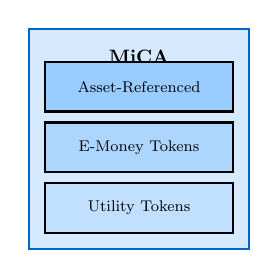
\begin{tikzpicture}[scale=0.7, transform shape]
% MiCA structure
\draw[thick, dfblue, fill=dflightblue4] (0,0) rectangle (4,4);
\node at (2,3.5) {\textbf{MiCA}};

\draw[thick, fill=dflightblue3] (0.3,0.3) rectangle (3.7,1.2);
\node[font=\footnotesize] at (2,0.75) {Utility Tokens};

\draw[thick, fill=dflightblue2] (0.3,1.4) rectangle (3.7,2.3);
\node[font=\footnotesize] at (2,1.85) {E-Money Tokens};

\draw[thick, fill=dflightblue] (0.3,2.5) rectangle (3.7,3.4);
\node[font=\footnotesize] at (2,2.95) {Asset-Referenced};
\end{tikzpicture}

\vspace{3mm}
\footnotesize
\textbf{Not covered:}\\
DeFi, NFTs (mostly), CBDCs
\end{column}
\end{columns}
\end{frame}

\begin{frame}{MiCA: Stablecoin Rules}
\begin{columns}[T]
\begin{column}{0.48\textwidth}
\textbf{Asset-Referenced Tokens (ARTs):}
\begin{itemize}
\item Backed by multiple assets
\item Issuer must be authorized
\item Reserve requirements
\item No interest payments
\item If ``significant'': stricter rules
\end{itemize}

\vspace{3mm}
\textbf{E-Money Tokens (EMTs):}
\begin{itemize}
\item Single fiat currency reference
\item Must be e-money institution
\item 1:1 redemption rights
\item Segregated reserves
\end{itemize}
\end{column}
\begin{column}{0.48\textwidth}
\begin{alertblock}{Significance Thresholds}
``Significant'' ART/EMT if:
\begin{itemize}
\item 10M+ holders
\item \EUR{}5B+ market cap
\item 2.5M+ daily transactions
\item \EUR{}500M+ daily value
\end{itemize}
Higher capital, stricter oversight.
\end{alertblock}

\vspace{3mm}
\textbf{Impact on USDT/USDC:}\\
Must comply or delist from EU exchanges.
\end{column}
\end{columns}
\end{frame}

\begin{frame}{Asia: Diverse Approaches}
\begin{center}
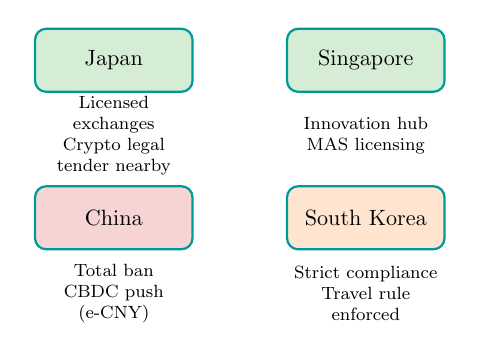
\begin{tikzpicture}[scale=0.8, transform shape]
% Map representation
\node (japan) [blockchain, minimum width=2.5cm, fill=dfgreen!20] {Japan};
\node (singapore) [blockchain, right of=japan, node distance=4cm, minimum width=2.5cm, fill=dfgreen!20] {Singapore};
\node (china) [blockchain, below of=japan, node distance=2.5cm, minimum width=2.5cm, fill=dfred!20] {China};
\node (korea) [blockchain, below of=singapore, node distance=2.5cm, minimum width=2.5cm, fill=dforange!20] {South Korea};

% Labels
\node[below of=japan, node distance=1.2cm, font=\footnotesize, text width=2.5cm, align=center] {Licensed exchanges\\Crypto legal tender nearby};
\node[below of=singapore, node distance=1.2cm, font=\footnotesize, text width=2.5cm, align=center] {Innovation hub\\MAS licensing};
\node[below of=china, node distance=1.2cm, font=\footnotesize, text width=2.5cm, align=center] {Total ban\\CBDC push (e-CNY)};
\node[below of=korea, node distance=1.2cm, font=\footnotesize, text width=2.5cm, align=center] {Strict compliance\\Travel rule enforced};
\end{tikzpicture}
\end{center}
\end{frame}

\begin{frame}{China: Complete Ban + CBDC}
\begin{columns}[T]
\begin{column}{0.48\textwidth}
\textbf{What's Banned:}
\begin{itemize}
\item Cryptocurrency trading
\item Crypto mining (since 2021)
\item ICOs
\item Crypto exchanges
\item Providing crypto services
\end{itemize}

\vspace{3mm}
\textbf{Penalties:}
\begin{itemize}
\item Criminal prosecution possible
\item Businesses shut down
\item Mining operations seized
\end{itemize}
\end{column}
\begin{column}{0.48\textwidth}
\textbf{Digital Yuan (e-CNY):}
\begin{itemize}
\item Central Bank Digital Currency
\item Controlled by PBoC
\item Two-tier distribution
\item Programmable money
\item Pilot programs in major cities
\end{itemize}

\vspace{3mm}
\begin{alertblock}{The Strategy}
Ban decentralized crypto, promote centralized CBDC. Maximum control, full surveillance.
\end{alertblock}
\end{column}
\end{columns}
\end{frame}

\begin{frame}{Regulatory Comparison Matrix}
\begin{center}
\renewcommand{\arraystretch}{1.2}
\footnotesize
\begin{tabular}{|l|c|c|c|c|}
\hline
\textbf{Aspect} & \textbf{US} & \textbf{EU (MiCA)} & \textbf{Singapore} & \textbf{China} \\
\hline
Crypto trading & Varies & Licensed & Licensed & \textcolor{dfred}{Banned} \\
\hline
Token issuance & Case-by-case & Whitepaper & Licensed & \textcolor{dfred}{Banned} \\
\hline
Stablecoins & Unclear & Regulated & Licensed & \textcolor{dfred}{Banned} \\
\hline
DeFi & Unclear & Unclear & Evolving & \textcolor{dfred}{Banned} \\
\hline
NFTs & Unclear & Mostly exempt & Evolving & Gray area \\
\hline
CBDC & Researching & Exploring & Exploring & \textcolor{dfgreen}{Live} \\
\hline
Clarity & \textcolor{dfred}{Low} & \textcolor{dfgreen}{High} & \textcolor{dforange}{Medium} & \textcolor{dfgreen}{High (ban)} \\
\hline
\end{tabular}
\end{center}

\vspace{3mm}
\begin{block}{Key Insight}
Regulatory arbitrage is real. Projects choose jurisdictions strategically. Clear rules (even strict ones) often preferred over uncertainty.
\end{block}
\end{frame}

\begin{frame}{The Travel Rule}
\begin{columns}[T]
\begin{column}{0.55\textwidth}
\textbf{What is it?}\\
FATF requirement: Virtual Asset Service Providers (VASPs) must share sender/receiver information for transfers above thresholds.

\vspace{3mm}
\textbf{Information Required:}
\begin{itemize}
\item Sender name
\item Sender account number
\item Sender address or ID
\item Beneficiary name
\item Beneficiary account number
\end{itemize}

\vspace{3mm}
\textbf{Thresholds:}
\begin{itemize}
\item US: \$3,000+
\item EU: \EUR{}0 (all transfers!)
\item FATF guidance: \$1,000
\end{itemize}
\end{column}
\begin{column}{0.42\textwidth}
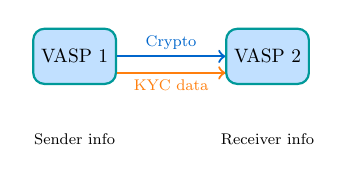
\begin{tikzpicture}[scale=0.7, transform shape, node distance=2cm]
% Travel rule flow
\node (vasp1) [blockchain, minimum width=1.5cm] {VASP 1};
\node (vasp2) [blockchain, right of=vasp1, node distance=3.5cm, minimum width=1.5cm] {VASP 2};

\draw[->, thick, dfblue] (vasp1) -- node[above, font=\footnotesize] {Crypto} (vasp2);
\draw[->, thick, dforange] ([yshift=-3mm]vasp1.east) -- node[below, font=\footnotesize] {KYC data} ([yshift=-3mm]vasp2.west);

\node[below of=vasp1, node distance=1.5cm, font=\footnotesize] {Sender info};
\node[below of=vasp2, node distance=1.5cm, font=\footnotesize] {Receiver info};
\end{tikzpicture}

\vspace{5mm}
\begin{alertblock}{DeFi Challenge}
How do you apply Travel Rule to non-custodial wallets and DEXs?
\end{alertblock}
\end{column}
\end{columns}
\end{frame}

\begin{frame}{DeFi Regulatory Challenges}
\begin{columns}[T]
\begin{column}{0.48\textwidth}
\textbf{The Fundamental Problem:}
\begin{itemize}
\item Who is the ``operator''?
\item Where is it located?
\item Who do you regulate?
\item How do you enforce?
\end{itemize}

\vspace{3mm}
\textbf{Potential Targets:}
\begin{itemize}
\item Frontend interfaces
\item Token holders with governance power
\item Core developers
\item Infrastructure providers
\end{itemize}
\end{column}
\begin{column}{0.48\textwidth}
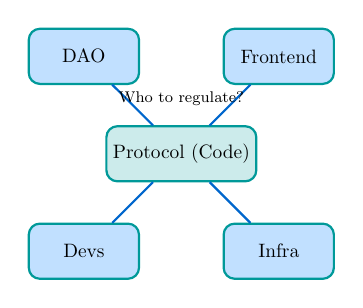
\begin{tikzpicture}[scale=0.7, transform shape]
% DeFi structure
\node (protocol) [blockchain, minimum width=2.5cm, fill=dfteal!20] {Protocol (Code)};
\node (governance) [blockchain, above left of=protocol, node distance=2.5cm, minimum width=2cm] {DAO};
\node (frontend) [blockchain, above right of=protocol, node distance=2.5cm, minimum width=2cm] {Frontend};
\node (devs) [blockchain, below left of=protocol, node distance=2.5cm, minimum width=2cm] {Devs};
\node (infra) [blockchain, below right of=protocol, node distance=2.5cm, minimum width=2cm] {Infra};

\draw[thick, dfblue] (governance) -- (protocol);
\draw[thick, dfblue] (frontend) -- (protocol);
\draw[thick, dfblue] (devs) -- (protocol);
\draw[thick, dfblue] (infra) -- (protocol);

\node[above of=protocol, node distance=1cm, font=\footnotesize] {Who to regulate?};
\end{tikzpicture}
\end{column}
\end{columns}

\vspace{3mm}
\begin{block}{Emerging Approach}
Target the chokepoints: fiat on/off ramps, centralized frontends, infrastructure providers.
\end{block}
\end{frame}

\begin{frame}{Case Study: Tornado Cash Sanctions}
\begin{columns}[T]
\begin{column}{0.55\textwidth}
\textbf{What Happened (Aug 2022):}
\begin{itemize}
\item US Treasury sanctioned Tornado Cash
\item Smart contract addresses added to OFAC list
\item Developer arrested in Netherlands
\item First time: CODE itself sanctioned
\end{itemize}

\vspace{3mm}
\textbf{Consequences:}
\begin{itemize}
\item GitHub removed repo
\item Circle froze USDC in addresses
\item Exchanges blocked deposits
\item Alchemy/Infura blocked RPC access
\end{itemize}
\end{column}
\begin{column}{0.42\textwidth}
\begin{alertblock}{Legal Questions}
\begin{itemize}
\item Can you sanction open-source code?
\item Is running a mixer illegal?
\item What about privacy rights?
\item First Amendment implications?
\end{itemize}
\end{alertblock}

\vspace{3mm}
\textbf{Outcome:}\\
Court ruled some sanctions overreach (2024). Case ongoing.
\end{column}
\end{columns}
\end{frame}

\begin{frame}{Discussion: Regulatory Philosophy}
\begin{columns}[T]
\begin{column}{0.48\textwidth}
\textbf{Argument for Strict Regulation:}
\begin{itemize}
\item Protect consumers from fraud
\item Prevent money laundering
\item Ensure financial stability
\item Level playing field with TradFi
\item Accountability for failures
\end{itemize}
\end{column}
\begin{column}{0.48\textwidth}
\textbf{Argument for Light Touch:}
\begin{itemize}
\item Enable innovation
\item Avoid regulatory arbitrage
\item Code is speech (1st Amendment)
\item Self-sovereignty rights
\item Regulation kills jobs
\end{itemize}
\end{column}
\end{columns}

\vspace{5mm}
\begin{block}{Discussion Questions}
\begin{itemize}
\item Should DeFi protocols be regulated like banks?
\item Is ``code is law'' compatible with rule of law?
\item What's the right balance for stablecoins?
\item Where would you launch a crypto startup?
\end{itemize}
\end{block}
\end{frame}

% =====================================================================
% SECTION 5.3: DAO GOVERNANCE
% =====================================================================
\section{5.3 DAO Governance}

\begin{frame}{Topic 5.3: Governance in Decentralized Systems}
\begin{center}
\textbf{\Large DAOs and the Limits of Code}
\end{center}

\vspace{5mm}
\textbf{Learning Objectives:}
\begin{itemize}
\item Explain DAO governance mechanisms
\item Identify governance attack vectors
\item Evaluate tradeoffs between on-chain and off-chain governance
\item Understand why ``code is law'' is insufficient
\end{itemize}

\vspace{5mm}
\begin{block}{Hands-On Component}
Colab notebook (NB12) simulating a DAO vote---model different token distributions and observe how governance outcomes change with concentration of voting power.
\end{block}
\end{frame}

\begin{frame}{What is a DAO?}
\begin{columns}[T]
\begin{column}{0.48\textwidth}
\textbf{Decentralized Autonomous Organization:}
\begin{itemize}
\item Rules encoded in smart contracts
\item Decisions via token holder voting
\item Treasury managed on-chain
\item No traditional legal structure
\item ``Code is law'' philosophy
\end{itemize}

\vspace{3mm}
\textbf{Common Functions:}
\begin{itemize}
\item Protocol upgrades
\item Parameter changes
\item Treasury allocation
\item Grant distribution
\item Strategic direction
\end{itemize}
\end{column}
\begin{column}{0.48\textwidth}
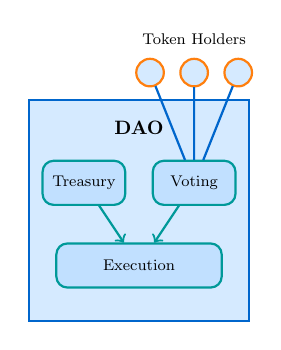
\begin{tikzpicture}[scale=0.7, transform shape]
% DAO structure
\draw[thick, dfblue, fill=dflightblue4] (0,0) rectangle (4,4);
\node at (2,3.5) {\textbf{DAO}};

% Components
\node (treasury) [blockchain, minimum width=1.5cm, minimum height=0.8cm] at (1,2.5) {\footnotesize Treasury};
\node (voting) [blockchain, minimum width=1.5cm, minimum height=0.8cm] at (3,2.5) {\footnotesize Voting};
\node (exec) [blockchain, minimum width=3cm, minimum height=0.8cm] at (2,1) {\footnotesize Execution};

\draw[->, thick, dfteal] (voting) -- (exec);
\draw[->, thick, dfteal] (treasury) -- (exec);

% Token holders
\node (h1) [transaction, above of=voting, node distance=2cm, minimum size=0.5cm] {};
\node (h2) [transaction, left of=h1, node distance=0.8cm, minimum size=0.5cm] {};
\node (h3) [transaction, right of=h1, node distance=0.8cm, minimum size=0.5cm] {};

\draw[thick, dfblue] (h1) -- (voting);
\draw[thick, dfblue] (h2) -- (voting);
\draw[thick, dfblue] (h3) -- (voting);

\node[above of=h1, node distance=0.6cm, font=\footnotesize] {Token Holders};
\end{tikzpicture}
\end{column}
\end{columns}
\end{frame}

\begin{frame}{DAO Governance Mechanisms}
\begin{columns}[T]
\begin{column}{0.48\textwidth}
\textbf{Token-Based Voting:}
\begin{itemize}
\item 1 token = 1 vote
\item Simple and transparent
\item But: plutocracy problem
\end{itemize}

\vspace{3mm}
\textbf{Quadratic Voting:}
\begin{itemize}
\item Cost increases quadratically
\item Reduces whale dominance
\item But: Sybil vulnerable
\end{itemize}

\vspace{3mm}
\textbf{Conviction Voting:}
\begin{itemize}
\item Votes accumulate over time
\item Rewards long-term alignment
\item But: slow decision-making
\end{itemize}
\end{column}
\begin{column}{0.48\textwidth}
\textbf{Delegation:}
\begin{itemize}
\item Delegate votes to experts
\item Addresses voter apathy
\item But: concentrates power
\end{itemize}

\vspace{3mm}
\textbf{Multi-sig:}
\begin{itemize}
\item N-of-M signers required
\item Fast execution
\item But: centralized trust
\end{itemize}

\vspace{3mm}
\textbf{Optimistic Governance:}
\begin{itemize}
\item Proposals pass unless vetoed
\item Efficient for routine decisions
\item But: requires active monitoring
\end{itemize}
\end{column}
\end{columns}
\end{frame}

\begin{frame}{The Plutocracy Problem}
\begin{center}
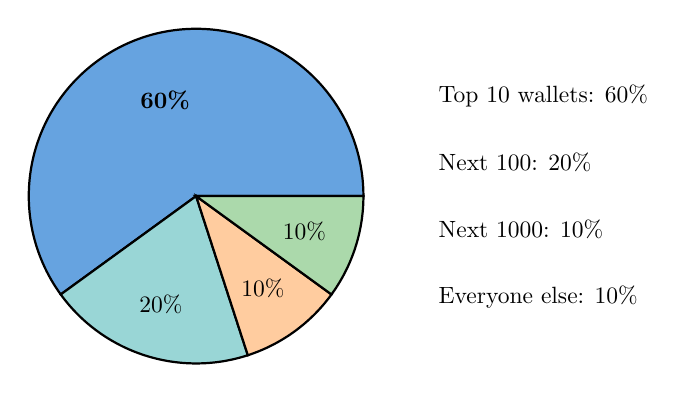
\begin{tikzpicture}[scale=0.85, transform shape]
% Token distribution pie chart
\draw[thick, fill=dfblue!60] (0,0) -- (0:2.5) arc (0:216:2.5) -- cycle;
\draw[thick, fill=dfteal!40] (0,0) -- (216:2.5) arc (216:288:2.5) -- cycle;
\draw[thick, fill=dforange!40] (0,0) -- (288:2.5) arc (288:324:2.5) -- cycle;
\draw[thick, fill=dfgreen!40] (0,0) -- (324:2.5) arc (324:360:2.5) -- cycle;

% Labels
\node at (108:1.5) {\textbf{60\%}};
\node at (252:1.7) {20\%};
\node at (306:1.7) {10\%};
\node at (342:1.7) {10\%};

% Legend
\node[right] at (3.5,1.5) {Top 10 wallets: 60\%};
\node[right] at (3.5,0.5) {Next 100: 20\%};
\node[right] at (3.5,-0.5) {Next 1000: 10\%};
\node[right] at (3.5,-1.5) {Everyone else: 10\%};
\end{tikzpicture}
\end{center}

\vspace{3mm}
\textbf{Reality:} Most DAOs have highly concentrated token distributions.\\
\textbf{Result:} A few whales control most decisions. ``Decentralized'' in name only.
\end{frame}

\begin{frame}{Governance Attack Vectors}
\begin{columns}[T]
\begin{column}{0.48\textwidth}
\textbf{Flash Loan Governance Attack:}
\begin{enumerate}
\item Borrow millions in governance tokens
\item Vote on malicious proposal
\item Execute immediately
\item Repay loan, keep profits
\end{enumerate}

\vspace{3mm}
\textbf{Beanstalk Attack (2022):}
\begin{itemize}
\item Flash borrowed \$1B in tokens
\item Passed proposal in one block
\item Drained \$182M from treasury
\item All in a single transaction
\end{itemize}
\end{column}
\begin{column}{0.48\textwidth}
\textbf{Other Attack Vectors:}
\begin{itemize}
\item \textbf{Vote buying:} Purchase votes off-chain
\item \textbf{Dark DAOs:} Coordinate attacks privately
\item \textbf{51\% attack:} Accumulate majority
\item \textbf{Delegation hijacking:} Compromise delegates
\item \textbf{Social engineering:} Manipulate key members
\end{itemize}

\vspace{3mm}
\begin{alertblock}{Key Insight}
Governance is the attack surface. Secure code means nothing if governance can change it.
\end{alertblock}
\end{column}
\end{columns}
\end{frame}

\begin{frame}{Case Study: Beanstalk Governance Attack}
\begin{center}
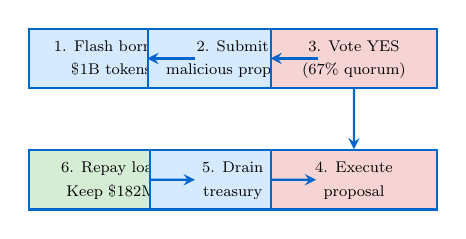
\begin{tikzpicture}[scale=0.7, transform shape, node distance=2.2cm]
% Attack sequence
\node (step1) [process, minimum width=3cm] {
\begin{tabular}{c}
\footnotesize 1. Flash borrow\\
\footnotesize \$1B tokens
\end{tabular}
};

\node (step2) [process, right of=step1, minimum width=3cm] {
\begin{tabular}{c}
\footnotesize 2. Submit\\
\footnotesize malicious proposal
\end{tabular}
};

\node (step3) [process, right of=step2, minimum width=3cm, fill=dfred!20] {
\begin{tabular}{c}
\footnotesize 3. Vote YES\\
\footnotesize (67\% quorum)
\end{tabular}
};

\node (step4) [process, below of=step1, minimum width=3cm, fill=dfgreen!20] {
\begin{tabular}{c}
\footnotesize 6. Repay loan\\
\footnotesize Keep \$182M
\end{tabular}
};

\node (step5) [process, below of=step2, minimum width=3cm] {
\begin{tabular}{c}
\footnotesize 5. Drain\\
\footnotesize treasury
\end{tabular}
};

\node (step6) [process, below of=step3, minimum width=3cm, fill=dfred!20] {
\begin{tabular}{c}
\footnotesize 4. Execute\\
\footnotesize proposal
\end{tabular}
};

\draw[arrow] (step1) -- (step2);
\draw[arrow] (step2) -- (step3);
\draw[arrow] (step3) -- (step6);
\draw[arrow] (step6) -- (step5);
\draw[arrow] (step5) -- (step4);
\end{tikzpicture}
\end{center}

\vspace{3mm}
\textbf{Critical flaw:} No time delay between vote and execution.\\
\textbf{Fix:} Timelocks, snapshot voting, flash loan protection.
\end{frame}

\begin{frame}{Governance Defenses}
\begin{columns}[T]
\begin{column}{0.48\textwidth}
\textbf{Timelocks:}
\begin{itemize}
\item Delay between approval and execution
\item Gives time to react to attacks
\item Standard: 24-48 hours minimum
\end{itemize}

\vspace{3mm}
\textbf{Vote Escrow:}
\begin{itemize}
\item Lock tokens to vote (veTokens)
\item Longer lock = more voting power
\item Prevents flash loan attacks
\end{itemize}

\vspace{3mm}
\textbf{Snapshot Voting:}
\begin{itemize}
\item Balance at specific block height
\item Cannot borrow tokens after snapshot
\end{itemize}
\end{column}
\begin{column}{0.48\textwidth}
\textbf{Quorum Requirements:}
\begin{itemize}
\item Minimum participation threshold
\item Higher for critical decisions
\item Risk: voter apathy blocks everything
\end{itemize}

\vspace{3mm}
\textbf{Guardian/Veto Power:}
\begin{itemize}
\item Multi-sig can block malicious proposals
\item Centralization tradeoff
\item ``Emergency brake''
\end{itemize}

\vspace{3mm}
\textbf{Optimistic Execution:}
\begin{itemize}
\item Proposals pass unless vetoed
\item Challenge period for objections
\end{itemize}
\end{column}
\end{columns}
\end{frame}

\begin{frame}{On-Chain vs. Off-Chain Governance}
\begin{center}
\renewcommand{\arraystretch}{1.3}
\begin{tabular}{|l|c|c|}
\hline
\textbf{Aspect} & \textbf{On-Chain} & \textbf{Off-Chain} \\
\hline
Binding & Automatic execution & Requires implementation \\
\hline
Transparency & Fully verifiable & Forum/snapshot \\
\hline
Cost & Gas fees & Usually free \\
\hline
Speed & Blockchain constrained & Faster iteration \\
\hline
Flexibility & Rigid (code) & Adaptable \\
\hline
Attacks & Flash loans, 51\% & Social, coordination \\
\hline
Examples & Compound, Uniswap & Bitcoin, Ethereum L1 \\
\hline
\end{tabular}
\end{center}

\vspace{3mm}
\begin{block}{Hybrid Approaches}
Most successful DAOs use both: off-chain discussion/signaling, on-chain execution with safeguards.
\end{block}
\end{frame}

\begin{frame}{The Voter Apathy Problem}
\begin{columns}[T]
\begin{column}{0.55\textwidth}
\textbf{Reality of DAO Participation:}
\begin{itemize}
\item Typical turnout: 1-5\% of tokens
\item Most token holders never vote
\item Few wallets dominate decisions
\item Governance fatigue is real
\end{itemize}

\vspace{3mm}
\textbf{Why People Don't Vote:}
\begin{itemize}
\item Gas costs (on-chain)
\item Time to understand proposals
\item Rational ignorance (1 vote doesn't matter)
\item Token holders $\neq$ users
\end{itemize}
\end{column}
\begin{column}{0.42\textwidth}
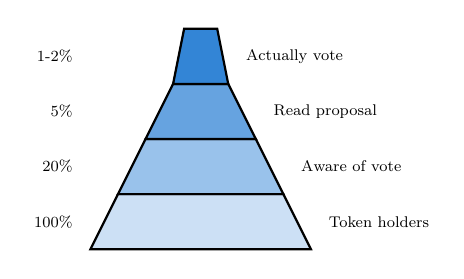
\begin{tikzpicture}[scale=0.7, transform shape]
% Participation funnel
\draw[thick, fill=dfblue!20] (0,0) -- (4,0) -- (3.5,1) -- (0.5,1) -- cycle;
\draw[thick, fill=dfblue!40] (0.5,1) -- (3.5,1) -- (3,2) -- (1,2) -- cycle;
\draw[thick, fill=dfblue!60] (1,2) -- (3,2) -- (2.5,3) -- (1.5,3) -- cycle;
\draw[thick, fill=dfblue!80] (1.5,3) -- (2.5,3) -- (2.3,4) -- (1.7,4) -- cycle;

\node[right, font=\footnotesize] at (4.2,0.5) {Token holders};
\node[right, font=\footnotesize] at (3.7,1.5) {Aware of vote};
\node[right, font=\footnotesize] at (3.2,2.5) {Read proposal};
\node[right, font=\footnotesize] at (2.7,3.5) {Actually vote};

\node[left, font=\footnotesize] at (-0.2,0.5) {100\%};
\node[left, font=\footnotesize] at (-0.2,1.5) {20\%};
\node[left, font=\footnotesize] at (-0.2,2.5) {5\%};
\node[left, font=\footnotesize] at (-0.2,3.5) {1-2\%};
\end{tikzpicture}
\end{column}
\end{columns}
\end{frame}

\begin{frame}{``Code is Law'' vs. Rule of Law}
\begin{columns}[T]
\begin{column}{0.48\textwidth}
\textbf{``Code is Law'' Philosophy:}
\begin{itemize}
\item Smart contract IS the agreement
\item No external intervention
\item Predictable, immutable
\item ``If the code allows it, it's allowed''
\end{itemize}

\vspace{3mm}
\textbf{The DAO Hack Challenge:}
\begin{itemize}
\item Hacker used code as designed
\item Was it theft or legitimate use?
\item Ethereum community chose to fork
\item ``Code is law'' violated by humans
\end{itemize}
\end{column}
\begin{column}{0.48\textwidth}
\textbf{Traditional Rule of Law:}
\begin{itemize}
\item Intent matters (mens rea)
\item Fairness considerations
\item Courts interpret disputes
\item Law evolves with society
\end{itemize}

\vspace{3mm}
\begin{alertblock}{The Tension}
Code cannot encode intent, fairness, or context. Pure ``code is law'' may be unjust. But human intervention undermines decentralization.
\end{alertblock}
\end{column}
\end{columns}
\end{frame}

\begin{frame}{Hands-On: DAO Voting Simulation (NB12)}
\begin{center}
\textbf{\Large Model How Token Distribution Affects Governance}
\end{center}

\vspace{5mm}
\textbf{In the Colab notebook, we will:}
\begin{enumerate}
\item Create token distributions with varying concentration
\item Simulate voting on proposals
\item Calculate Gini coefficients for voting power
\item Test attack scenarios (whale dominance, flash loans)
\item Explore defense mechanisms (quadratic voting, delegation)
\end{enumerate}

\vspace{5mm}
\begin{block}{Access the Notebook}
\texttt{day\_05/notebooks/NB12\_DAO\_Governance.ipynb}

\vspace{2mm}
\footnotesize See how 1 whale with 51\% can override 10,000 small holders.
\end{block}

\bottomnote{Time: 20-25 minutes for guided exploration}
\end{frame}

\begin{frame}{Discussion: Governance Tradeoffs}
\begin{columns}[T]
\begin{column}{0.48\textwidth}
\textbf{Questions to Consider:}
\begin{enumerate}
\item Is plutocracy inherent to token voting?
\item Should DAOs have constitutions?
\item When is centralization acceptable?
\item Can code ever fully replace human judgment?
\end{enumerate}
\end{column}
\begin{column}{0.48\textwidth}
\textbf{Key Takeaways:}
\begin{itemize}
\item Governance IS the attack surface
\item Token distribution = power distribution
\item ``Decentralized'' often isn't
\item Hybrid models emerging
\end{itemize}
\end{column}
\end{columns}

\vspace{5mm}
\begin{alertblock}{The Governance Trilemma}
You can optimize for two of three: \textbf{Decentralization}, \textbf{Efficiency}, \textbf{Security}. Pick which one to sacrifice.
\end{alertblock}
\end{frame}

% =====================================================================
% SECTION 5.4: PRIVACY, SURVEILLANCE, AND FINANCIAL INCLUSION
% =====================================================================
\section{5.4 Privacy, Surveillance, and Financial Inclusion}

\begin{frame}{Topic 5.4: Privacy, Surveillance, and Financial Inclusion}
\begin{center}
\textbf{\Large Who Benefits and Who Is Harmed?}
\end{center}

\vspace{5mm}
\textbf{Learning Objectives:}
\begin{itemize}
\item Articulate the privacy-transparency tradeoff
\item Evaluate financial inclusion claims critically
\item Form a reasoned position on surveillance in finance
\item Understand who benefits from different design choices
\end{itemize}

\vspace{5mm}
\begin{block}{The Central Tension}
Digital finance creates unprecedented transparency (for regulation, trust) and unprecedented surveillance (of individuals, by states and corporations).
\end{block}
\end{frame}

\begin{frame}{The Privacy-Transparency Spectrum}
\begin{center}
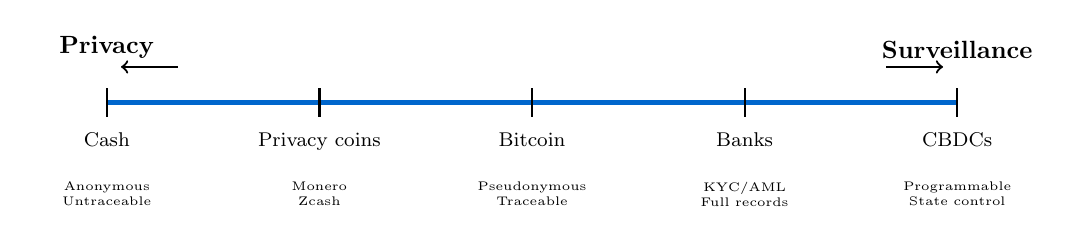
\begin{tikzpicture}[scale=0.9, transform shape]
% Spectrum line
\draw[ultra thick, dfblue] (0,0) -- (12,0);

% Markers
\foreach \x in {0,3,6,9,12} {
    \draw[thick] (\x,-0.2) -- (\x,0.2);
}

% Labels
\node[below] at (0,-0.3) {\footnotesize Cash};
\node[below] at (3,-0.3) {\footnotesize Privacy coins};
\node[below] at (6,-0.3) {\footnotesize Bitcoin};
\node[below] at (9,-0.3) {\footnotesize Banks};
\node[below] at (12,-0.3) {\footnotesize CBDCs};

% Arrow labels
\node[above] at (0,0.5) {\textbf{Privacy}};
\node[above] at (12,0.5) {\textbf{Surveillance}};
\draw[->, thick] (1,0.5) -- (0.2,0.5);
\draw[->, thick] (11,0.5) -- (11.8,0.5);

% Descriptions below
\node[below, text width=2cm, align=center, font=\tiny] at (0,-1) {Anonymous\\Untraceable};
\node[below, text width=2cm, align=center, font=\tiny] at (3,-1) {Monero\\Zcash};
\node[below, text width=2cm, align=center, font=\tiny] at (6,-1) {Pseudonymous\\Traceable};
\node[below, text width=2cm, align=center, font=\tiny] at (9,-1) {KYC/AML\\Full records};
\node[below, text width=2cm, align=center, font=\tiny] at (12,-1) {Programmable\\State control};
\end{tikzpicture}
\end{center}

\vspace{5mm}
\textbf{Key question:} Where on this spectrum should financial systems be?
\end{frame}

\begin{frame}{Arguments for Financial Privacy}
\begin{columns}[T]
\begin{column}{0.48\textwidth}
\textbf{Individual Rights:}
\begin{itemize}
\item Financial data reveals beliefs, health, relationships
\item Surveillance chills free expression
\item Protection from domestic abuse
\item Competitive business information
\end{itemize}

\vspace{3mm}
\textbf{Historical Precedent:}
\begin{itemize}
\item Nazi Germany: bank records used for persecution
\item Authoritarian states freeze activist accounts
\item Corporate surveillance for profit
\end{itemize}
\end{column}
\begin{column}{0.48\textwidth}
\textbf{Fungibility Principle:}
\begin{itemize}
\item Money should be interchangeable
\item Tainted coins create second-class money
\item Privacy preserves fungibility
\end{itemize}

\vspace{3mm}
\begin{block}{Human Rights Perspective}
UN Declaration of Human Rights, Article 12:\\
``No one shall be subjected to arbitrary interference with his privacy.''
\end{block}
\end{column}
\end{columns}
\end{frame}

\begin{frame}{Arguments for Financial Transparency}
\begin{columns}[T]
\begin{column}{0.48\textwidth}
\textbf{Anti-Crime Rationale:}
\begin{itemize}
\item Money laundering enables crime
\item Terrorist financing
\item Tax evasion
\item Sanctions enforcement
\item Fraud detection
\end{itemize}

\vspace{3mm}
\textbf{Consumer Protection:}
\begin{itemize}
\item Dispute resolution
\item Fraud recovery
\item Accountability for institutions
\end{itemize}
\end{column}
\begin{column}{0.48\textwidth}
\textbf{Market Integrity:}
\begin{itemize}
\item Insider trading detection
\item Market manipulation prevention
\item Fair price discovery
\end{itemize}

\vspace{3mm}
\begin{alertblock}{The AML Argument}
\$800B-\$2T laundered annually. Transparency enables enforcement. ``Nothing to hide, nothing to fear.''
\end{alertblock}
\end{column}
\end{columns}
\end{frame}

\begin{frame}{CBDCs: The Ultimate Surveillance Tool?}
\begin{columns}[T]
\begin{column}{0.55\textwidth}
\textbf{CBDC Capabilities:}
\begin{itemize}
\item Complete transaction visibility
\item Programmable spending restrictions
\item Automatic tax collection
\item Expiring money (demurrage)
\item Geographic restrictions
\item Social credit integration
\end{itemize}

\vspace{3mm}
\textbf{China's e-CNY:}
\begin{itemize}
\item Real-time government visibility
\item Can be programmed for uses
\item Integrated with social systems
\item Pilot: 260M wallets
\end{itemize}
\end{column}
\begin{column}{0.42\textwidth}
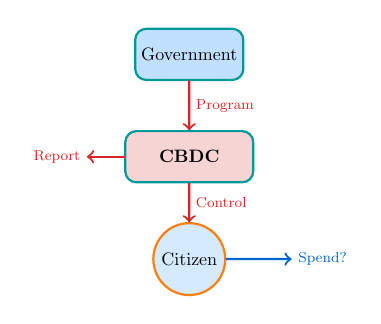
\begin{tikzpicture}[scale=0.65, transform shape]
% CBDC structure
\node (cbdc) [blockchain, minimum width=2.5cm, fill=dfred!20] {\textbf{CBDC}};
\node (gov) [blockchain, above of=cbdc, node distance=2cm, minimum width=2cm] {Government};
\node (citizen) [transaction, below of=cbdc, node distance=2cm] {Citizen};

\draw[->, thick, dfred] (cbdc) -- node[right, font=\footnotesize] {Control} (citizen);
\draw[->, thick, dfred] (gov) -- node[right, font=\footnotesize] {Program} (cbdc);
\draw[->, thick, dfblue] (citizen) -- ++(2,0) node[right, font=\footnotesize] {Spend?};
\draw[->, thick, dfred] (cbdc) -- ++(-2,0) node[left, font=\footnotesize] {Report};
\end{tikzpicture}

\vspace{3mm}
\begin{alertblock}{Dystopian Scenario}
Money that watches you, judges you, and can be remotely disabled.
\end{alertblock}
\end{column}
\end{columns}
\end{frame}

\begin{frame}{Privacy Technologies}
\begin{columns}[T]
\begin{column}{0.48\textwidth}
\textbf{Privacy Coins:}
\begin{itemize}
\item \textbf{Monero (XMR):} Ring signatures, stealth addresses
\item \textbf{Zcash (ZEC):} zk-SNARKs, shielded transactions
\item \textbf{Dash:} CoinJoin mixing
\end{itemize}

\vspace{3mm}
\textbf{Mixing Services:}
\begin{itemize}
\item Tornado Cash (sanctioned)
\item CoinJoin implementations
\item Tumbling services
\end{itemize}
\end{column}
\begin{column}{0.48\textwidth}
\textbf{Zero-Knowledge Proofs:}
\begin{itemize}
\item Prove something without revealing it
\item ``I'm over 18'' without showing ID
\item ``I have funds'' without showing balance
\end{itemize}

\vspace{3mm}
\begin{block}{zk-Proofs for Compliance}
Emerging: Prove you're not on sanctions list WITHOUT revealing identity. Privacy AND compliance.
\end{block}
\end{column}
\end{columns}
\end{frame}

\begin{frame}{The Financial Inclusion Promise}
\begin{columns}[T]
\begin{column}{0.55\textwidth}
\textbf{The Narrative:}
\begin{itemize}
\item 1.4 billion unbanked adults
\item Mobile phones everywhere
\item Crypto bypasses gatekeepers
\item ``Bank the unbanked''
\end{itemize}

\vspace{3mm}
\textbf{Success Stories:}
\begin{itemize}
\item M-Pesa in Kenya (FinTech)
\item Remittances via stablecoins
\item Bitcoin in El Salvador (controversial)
\item Microloans via DeFi
\end{itemize}
\end{column}
\begin{column}{0.42\textwidth}
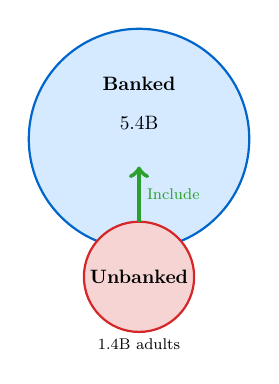
\begin{tikzpicture}[scale=0.7, transform shape]
% Inclusion diagram
\draw[thick, dfblue, fill=dflightblue4] (0,0) circle (2cm);
\node at (0,1) {\textbf{Banked}};
\node at (0,0.3) {5.4B};

\draw[thick, dfred, fill=dfred!20] (0,-2.5) circle (1cm);
\node at (0,-2.5) {\textbf{Unbanked}};
\node[below, font=\footnotesize] at (0,-3.5) {1.4B adults};

% Arrow
\draw[->, ultra thick, dfgreen] (0,-1.5) -- node[right, font=\footnotesize] {Include} (0,-0.5);
\end{tikzpicture}
\end{column}
\end{columns}
\end{frame}

\begin{frame}{The Financial Inclusion Critique}
\begin{columns}[T]
\begin{column}{0.48\textwidth}
\textbf{Barriers Remain:}
\begin{itemize}
\item Internet access required
\item Smartphone/device costs
\item Technical literacy
\item Language barriers
\item Volatility hurts the poor most
\end{itemize}

\vspace{3mm}
\textbf{Who Actually Benefits:}
\begin{itemize}
\item Tech-savvy early adopters
\item Those with capital to invest
\item Speculators and traders
\item Not primarily the unbanked
\end{itemize}
\end{column}
\begin{column}{0.48\textwidth}
\textbf{New Exclusions Created:}
\begin{itemize}
\item Complex UX excludes many
\item Gas fees price out small transactions
\item Scams disproportionately hurt naive users
\item Regulatory uncertainty creates risk
\end{itemize}

\vspace{3mm}
\begin{alertblock}{Critical Question}
Is crypto solving inclusion, or repackaging exclusion in new forms?
\end{alertblock}
\end{column}
\end{columns}
\end{frame}

\begin{frame}{Case Study: El Salvador Bitcoin Experiment}
\begin{columns}[T]
\begin{column}{0.55\textwidth}
\textbf{What Happened (Sept 2021):}
\begin{itemize}
\item Bitcoin made legal tender
\item \$30 Bitcoin airdrop to citizens
\item Government-backed Chivo wallet
\item Volcano-powered mining
\end{itemize}

\vspace{3mm}
\textbf{Stated Goals:}
\begin{itemize}
\item Financial inclusion (70\% unbanked)
\item Cheaper remittances (20\% of GDP)
\item Attract investment
\item Reduce dollar dependence
\end{itemize}
\end{column}
\begin{column}{0.42\textwidth}
\textbf{Results (2024):}
\begin{itemize}
\item Adoption: limited daily use
\item Remittances: mostly traditional
\item Volatility: government losses
\item IMF concerns
\item Tourism boost (crypto tourists)
\end{itemize}

\vspace{3mm}
\begin{block}{Verdict}
Mixed at best. Inclusion gains modest; volatility risks real; adoption limited to merchants near tourists.
\end{block}
\end{column}
\end{columns}
\end{frame}

\begin{frame}{Who Benefits? Who Is Harmed?}
\begin{center}
\renewcommand{\arraystretch}{1.3}
\begin{tabular}{|l|l|l|}
\hline
\textbf{Design Choice} & \textbf{Benefits} & \textbf{Harms} \\
\hline
Full transparency & Regulators, auditors & Privacy-seekers, dissidents \\
\hline
Full privacy & Individuals, activists & Law enforcement, victims \\
\hline
Pseudonymity (Bitcoin) & Moderate privacy & Linkability risk \\
\hline
CBDCs & Governments, AML & Individual autonomy \\
\hline
KYC requirements & Compliance, banks & Unbanked, privacy \\
\hline
Permissionless access & Underserved, censored & May enable crime \\
\hline
\end{tabular}
\end{center}

\vspace{3mm}
\begin{alertblock}{No Neutral Design}
Every architectural choice has distributional consequences. Technology is not neutral---it embeds values.
\end{alertblock}
\end{frame}

\begin{frame}{The Surveillance Capitalism Connection}
\begin{columns}[T]
\begin{column}{0.55\textwidth}
\textbf{Financial Data as Product:}
\begin{itemize}
\item Transaction data sold to advertisers
\item Credit scoring as control mechanism
\item Behavioral prediction markets
\item Insurance discrimination
\end{itemize}

\vspace{3mm}
\textbf{Corporate vs. State Surveillance:}
\begin{itemize}
\item PayPal, Visa see all transactions
\item Data shared with governments
\item No warrant needed for corporate data
\item ``Third-party doctrine'' in US
\end{itemize}
\end{column}
\begin{column}{0.42\textwidth}
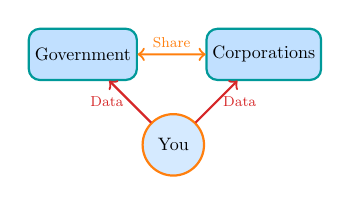
\begin{tikzpicture}[scale=0.65, transform shape]
% Surveillance triangle
\node (you) [transaction, minimum size=1.2cm] {You};
\node (corp) [blockchain, above right of=you, node distance=2.5cm, minimum width=2cm] {Corporations};
\node (gov) [blockchain, above left of=you, node distance=2.5cm, minimum width=2cm] {Government};

\draw[->, thick, dfred] (you) -- node[right, font=\footnotesize] {Data} (corp);
\draw[->, thick, dfred] (you) -- node[left, font=\footnotesize] {Data} (gov);
\draw[<->, thick, dforange] (corp) -- node[above, font=\footnotesize] {Share} (gov);
\end{tikzpicture}

\vspace{3mm}
\footnotesize
You are the product.\\
Your transactions are the data.\\
Privacy is the cost.
\end{column}
\end{columns}
\end{frame}

\begin{frame}{Emerging Privacy Solutions}
\begin{columns}[T]
\begin{column}{0.48\textwidth}
\textbf{Selective Disclosure:}
\begin{itemize}
\item Reveal only what's needed
\item Age verification without DOB
\item Solvency proof without balance
\item Compliance without surveillance
\end{itemize}

\vspace{3mm}
\textbf{Privacy-Preserving Compliance:}
\begin{itemize}
\item zk-proofs for sanctions screening
\item Encrypted transaction monitoring
\item Decentralized identity
\end{itemize}
\end{column}
\begin{column}{0.48\textwidth}
\textbf{Example: Proving Non-Sanction}
\begin{enumerate}
\item Hash your identity locally
\item Prove hash NOT on OFAC list
\item Zero-knowledge proof sent
\item Never reveal actual identity
\end{enumerate}

\vspace{3mm}
\begin{block}{The Vision}
Compliance without surveillance. Privacy AND legitimacy. Technically possible, politically challenging.
\end{block}
\end{column}
\end{columns}
\end{frame}

\begin{frame}{Discussion: Where Do You Stand?}
\begin{columns}[T]
\begin{column}{0.48\textwidth}
\textbf{Team Privacy Argues:}
\begin{itemize}
\item Privacy is a human right
\item Surveillance enables authoritarianism
\item Financial freedom requires anonymity
\item Technology should protect individuals
\end{itemize}
\end{column}
\begin{column}{0.48\textwidth}
\textbf{Team Transparency Argues:}
\begin{itemize}
\item Privacy enables crime
\item Society needs accountability
\item Victims deserve recourse
\item ``Sunlight is the best disinfectant''
\end{itemize}
\end{column}
\end{columns}

\vspace{5mm}
\begin{block}{Discussion Questions}
\begin{itemize}
\item Should there be a right to financial privacy?
\item Who gets to decide the tradeoff?
\item Is financial inclusion marketing or reality?
\item Would you use a CBDC?
\end{itemize}
\end{block}
\end{frame}

% =====================================================================
% DAY 5 SYNTHESIS
% =====================================================================
\section{Day 5 Synthesis}

\begin{frame}{Day 5 Synthesis}
\begin{columns}[T]
\begin{column}{0.48\textwidth}
\textbf{What We Covered:}
\begin{enumerate}
\item \textbf{Failures:} Technical, economic, human
\item \textbf{Regulation:} US fragmentation, EU MiCA, Asia divergence
\item \textbf{Governance:} DAO mechanisms and attacks
\item \textbf{Privacy:} Surveillance vs. autonomy tradeoffs
\end{enumerate}
\end{column}
\begin{column}{0.48\textwidth}
\textbf{Key Takeaways:}
\begin{itemize}
\item Failures are inevitable---design for them
\item Regulation shapes what survives
\item Governance IS the attack surface
\item Privacy vs. transparency is political
\item Financial inclusion: promise vs. reality
\end{itemize}
\end{column}
\end{columns}

\vspace{5mm}
\begin{alertblock}{Day Arc}
What fails (5.1) $\rightarrow$ Who governs from outside (5.2) $\rightarrow$ Who governs from inside (5.3) $\rightarrow$ Who benefits and who is harmed (5.4)
\end{alertblock}
\end{frame}

\begin{frame}{The Risk Framework}
\begin{center}
\textbf{\Large For Any Digital Finance System, Ask:}
\end{center}

\vspace{5mm}
\begin{enumerate}
\item \textbf{Technical:} What can go wrong with the code/infrastructure?
\item \textbf{Economic:} What incentive attacks are possible?
\item \textbf{Human:} Who has power and might abuse it?
\item \textbf{Regulatory:} What jurisdiction risks exist?
\item \textbf{Governance:} Who decides changes, and how?
\item \textbf{Privacy:} Who sees what, and what can they do with it?
\item \textbf{Inclusion:} Who benefits, who is excluded, who is harmed?
\end{enumerate}

\vspace{5mm}
\begin{block}{The Critical Mindset}
Move from ``what can this do?'' to ``what can go wrong, and for whom?''
\end{block}
\end{frame}

\begin{frame}{Looking Ahead: Day 6}
\begin{center}
\textbf{\Large Convergence and the Future: Where Is Digital Finance Going?}
\end{center}

\vspace{5mm}
\textbf{We'll explore:}
\begin{itemize}
\item TradFi + DeFi convergence
\item Institutional adoption
\item CBDCs and the future of money
\item AI + Finance integration
\item Your role in shaping this future
\end{itemize}

\vspace{5mm}
\textbf{Preparation:}
\begin{itemize}
\item Complete Day 5 notebooks (NB11, NB12)
\item Reflect: What would YOU build?
\item Think: What regulations would YOU write?
\end{itemize}
\end{frame}

\begin{frame}{Resources}
\textbf{Notebooks:}
\begin{itemize}
\item \texttt{day\_05/notebooks/NB11\_DeFi\_Exploits.ipynb}
\item \texttt{day\_05/notebooks/NB12\_DAO\_Governance.ipynb}
\end{itemize}

\vspace{3mm}
\textbf{Further Reading:}
\begin{itemize}
\item EU MiCA Regulation (EUR-Lex)
\item FATF Guidance on Virtual Assets
\item Chainalysis Crypto Crime Report
\item Vitalik Buterin on Governance
\end{itemize}

\vspace{3mm}
\textbf{Concepts to Review:}
\begin{itemize}
\item Reentrancy attacks, flash loans
\item Howey Test, MiCA categories
\item DAO governance mechanisms
\item Privacy-transparency tradeoff
\end{itemize}
\end{frame}

\begin{frame}{}
\begin{center}
\vspace{2cm}
{\Huge \textbf{Questions?}}

\vspace{1cm}
{\Large Day 5: Risk, Regulation, and the Dark Side}

\vspace{0.5cm}
{\large What Goes Wrong and Who Decides What's Allowed}

\vspace{1.5cm}
\textcolor{dfgray}{Next: Day 6 -- Convergence and the Future}
\end{center}
\end{frame}

\end{document}
